\documentclass[compress]{beamer}
\usepackage{ifthen,verbatim}

\title{Muon HIP Baseline Results}
\author{Jim Pivarski, Alexei Safonov}
\institute{Texas A\&M University}
\date{23 May, 2008}

\newcommand{\isnote}{}
\xdefinecolor{lightyellow}{rgb}{1.,1.,0.25}
\xdefinecolor{darkblue}{rgb}{0.1,0.1,0.7}

%% Uncomment this to get annotations
%% \def\notes{\addtocounter{page}{-1}
%%            \renewcommand{\isnote}{*}
%% 	   \beamertemplateshadingbackground{lightyellow}{white}
%%            \begin{frame}
%%            \frametitle{Notes for the previous page (page \insertpagenumber)}
%%            \itemize}
%% \def\endnotes{\enditemize
%% 	      \end{frame}
%%               \beamertemplateshadingbackground{white}{white}
%%               \renewcommand{\isnote}{}}

%% Uncomment this to not get annotations
\def\notes{\comment}
\def\endnotes{\endcomment}

\setbeamertemplate{navigation symbols}{}
\setbeamertemplate{headline}{\mbox{ } \hfill
\begin{minipage}{5.5 cm}
\vspace{-0.75 cm} \small
\end{minipage} \hfill
\begin{minipage}{4.5 cm}
\vspace{-0.75 cm} \small
\begin{flushright}
\ifthenelse{\equal{\insertpagenumber}{1}}{}{Jim Pivarski \hspace{0.2 cm} \insertpagenumber\isnote/\pageref{numpages}}
\end{flushright}
\end{minipage}\mbox{\hspace{0.2 cm}}\includegraphics[height=1 cm]{../cmslogo} \hspace{0.1 cm} \includegraphics[height=1 cm]{../tamulogo} \hspace{0.01 cm} \vspace{-1.05 cm}}

\begin{document}
\frame{\titlepage}

%% \begin{notes}
%% \item This is the annotated version of my talk.
%% \item If you want the version that I am presenting, download the one
%% labeled ``slides'' on Indico (or just ignore these yellow pages).
%% \item The annotated version is provided for extra detail and a written
%% record of comments that I intend to make orally.
%% \item Yellow notes refer to the content on the {\it previous} page.
%% \item All other slides are identical for the two versions.
%% \end{notes}

\begin{frame}
\frametitle{Basic story}
\small

\begin{itemize}\setlength{\itemsep}{0.1 cm}
\item Quality of MuonHIP alignment depends strongly on tracker alignment
\item S156 tracker alignment is good enough for a ``satisfactory'' muon alignment
\begin{itemize}
\item barrel $r\phi$ resolution strongly correlated with tracker alignment's $p_T$ results
\end{itemize}
\item Considered alternative schemes to include muon hits in track refit and iterate
\begin{itemize}
\item narrowed residuals distributions as expected
\item but the means are still imperfectly placed
\item converged slowly to the same result as one-step procedure
\end{itemize}
\item Results: all stations aligned in local $x$, and $\phi_z$, some in $y$
\begin{itemize}
\item all stations either improved or stayed the same; kept all corrections
\end{itemize}

\end{itemize}
%% \hspace{-0.83 cm} \textcolor{darkblue}{\Large Outline2}
\end{frame}

\begin{frame}
\frametitle{Barrel comparison $x$ (global $r\phi$)}
\small

Muon HIP barrel actual station 1: 680~$\mu$m

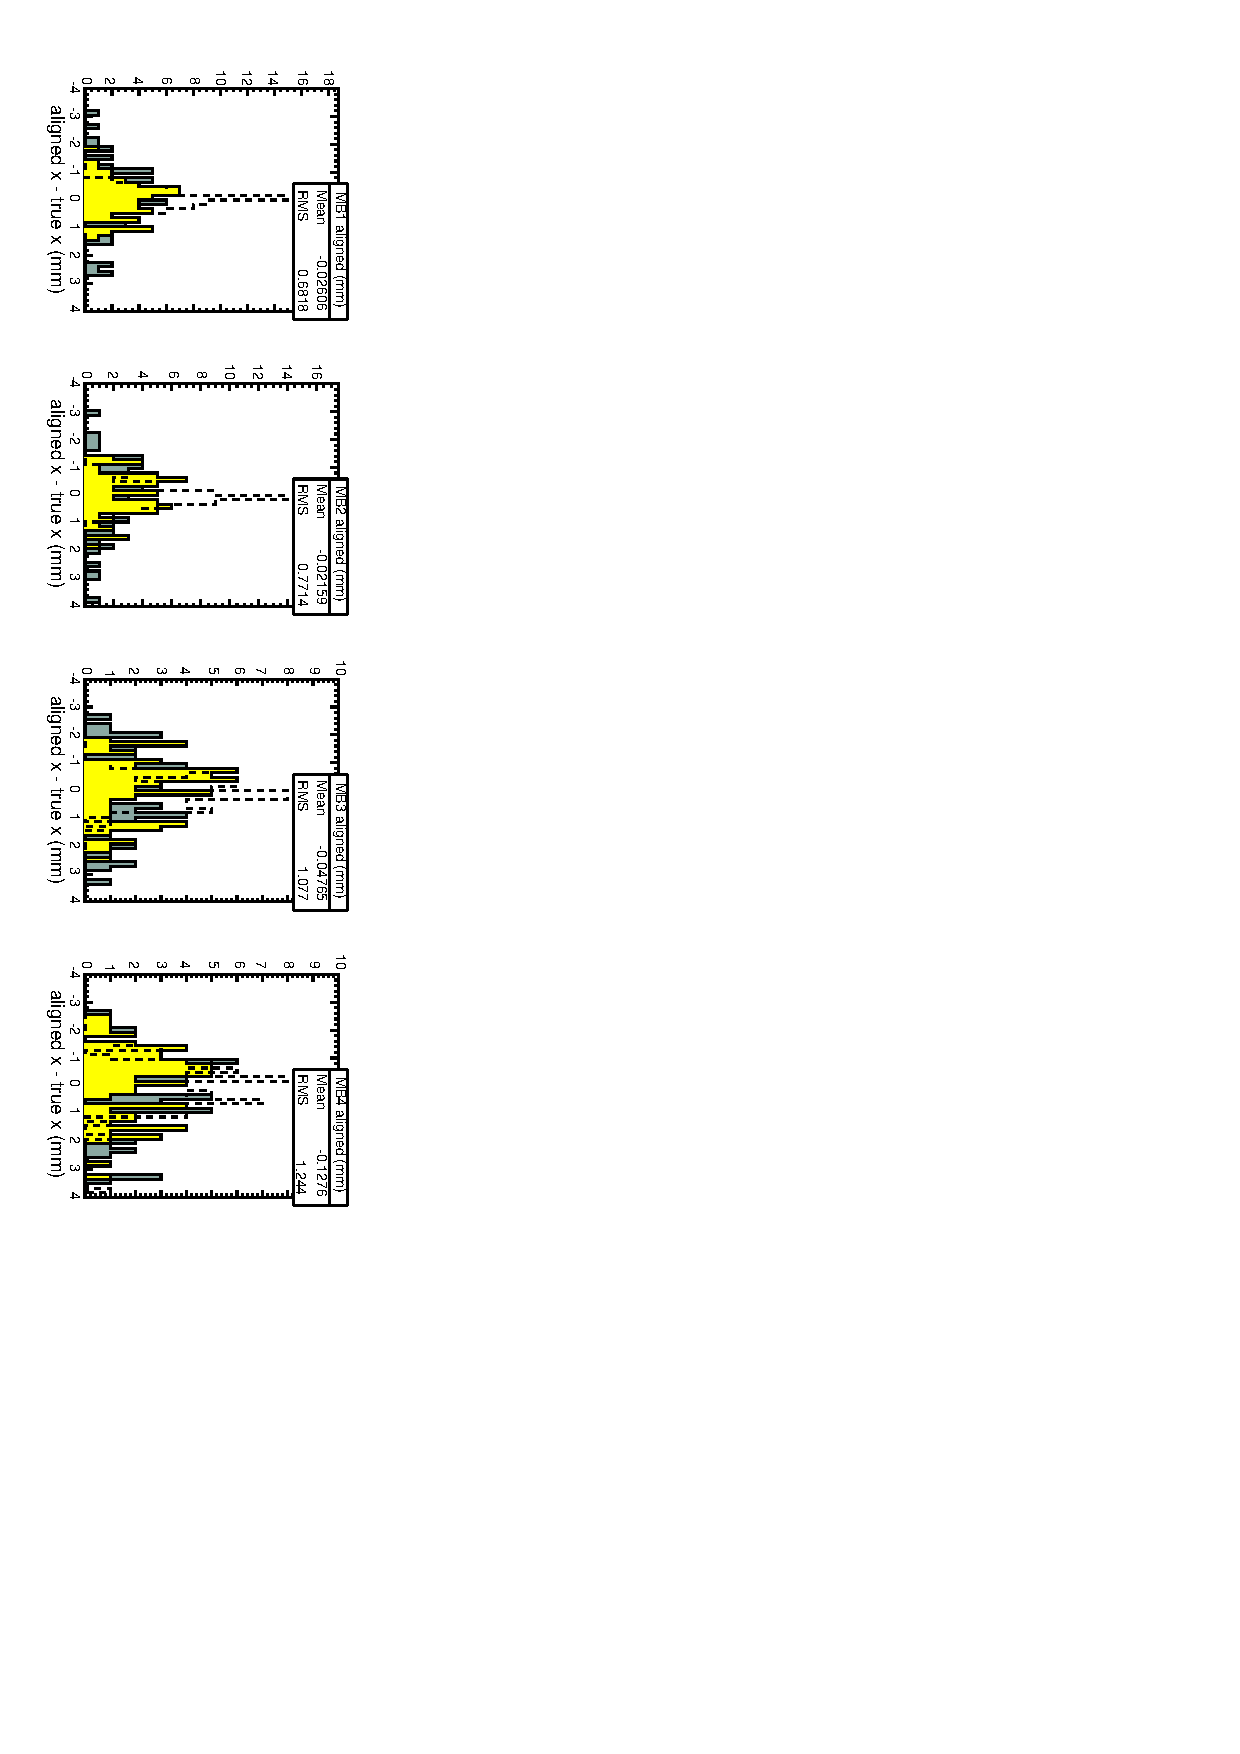
\includegraphics[height=\linewidth, angle=90]{S156_plots/muonhip_barrelx.pdf}

\vfill
MillePede barrel station 1: 1240~$\mu$m

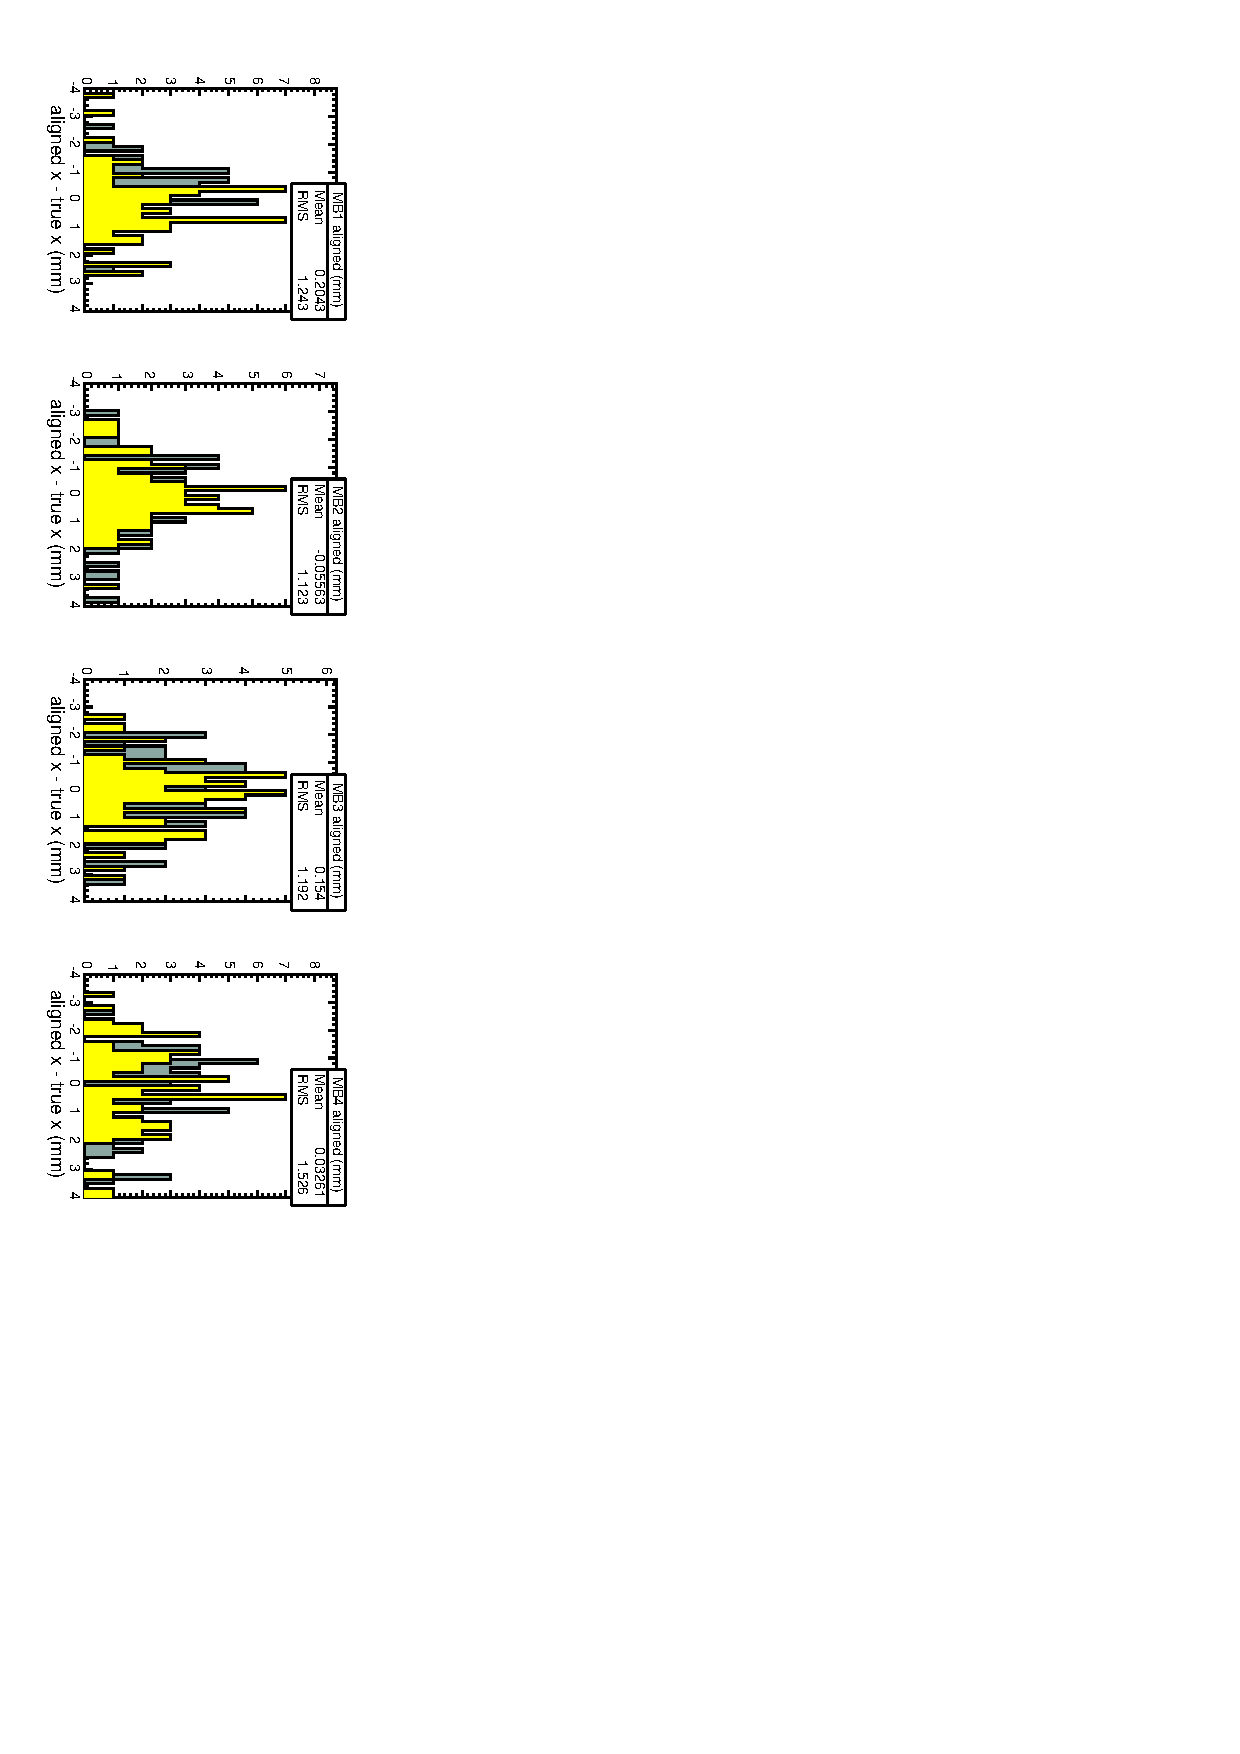
\includegraphics[height=\linewidth, angle=90]{S156_plots/millepede_barrelx.pdf}

\vfill
Filled grey is initial misalignment, filled yellow is actual new constants, \\ dashed line if tracker were perfect
\end{frame}

\begin{frame}
\frametitle{Barrel comparison $y$ (global $z$)}
\small

Muon HIP barrel actual station 1: 1840~$\mu$m

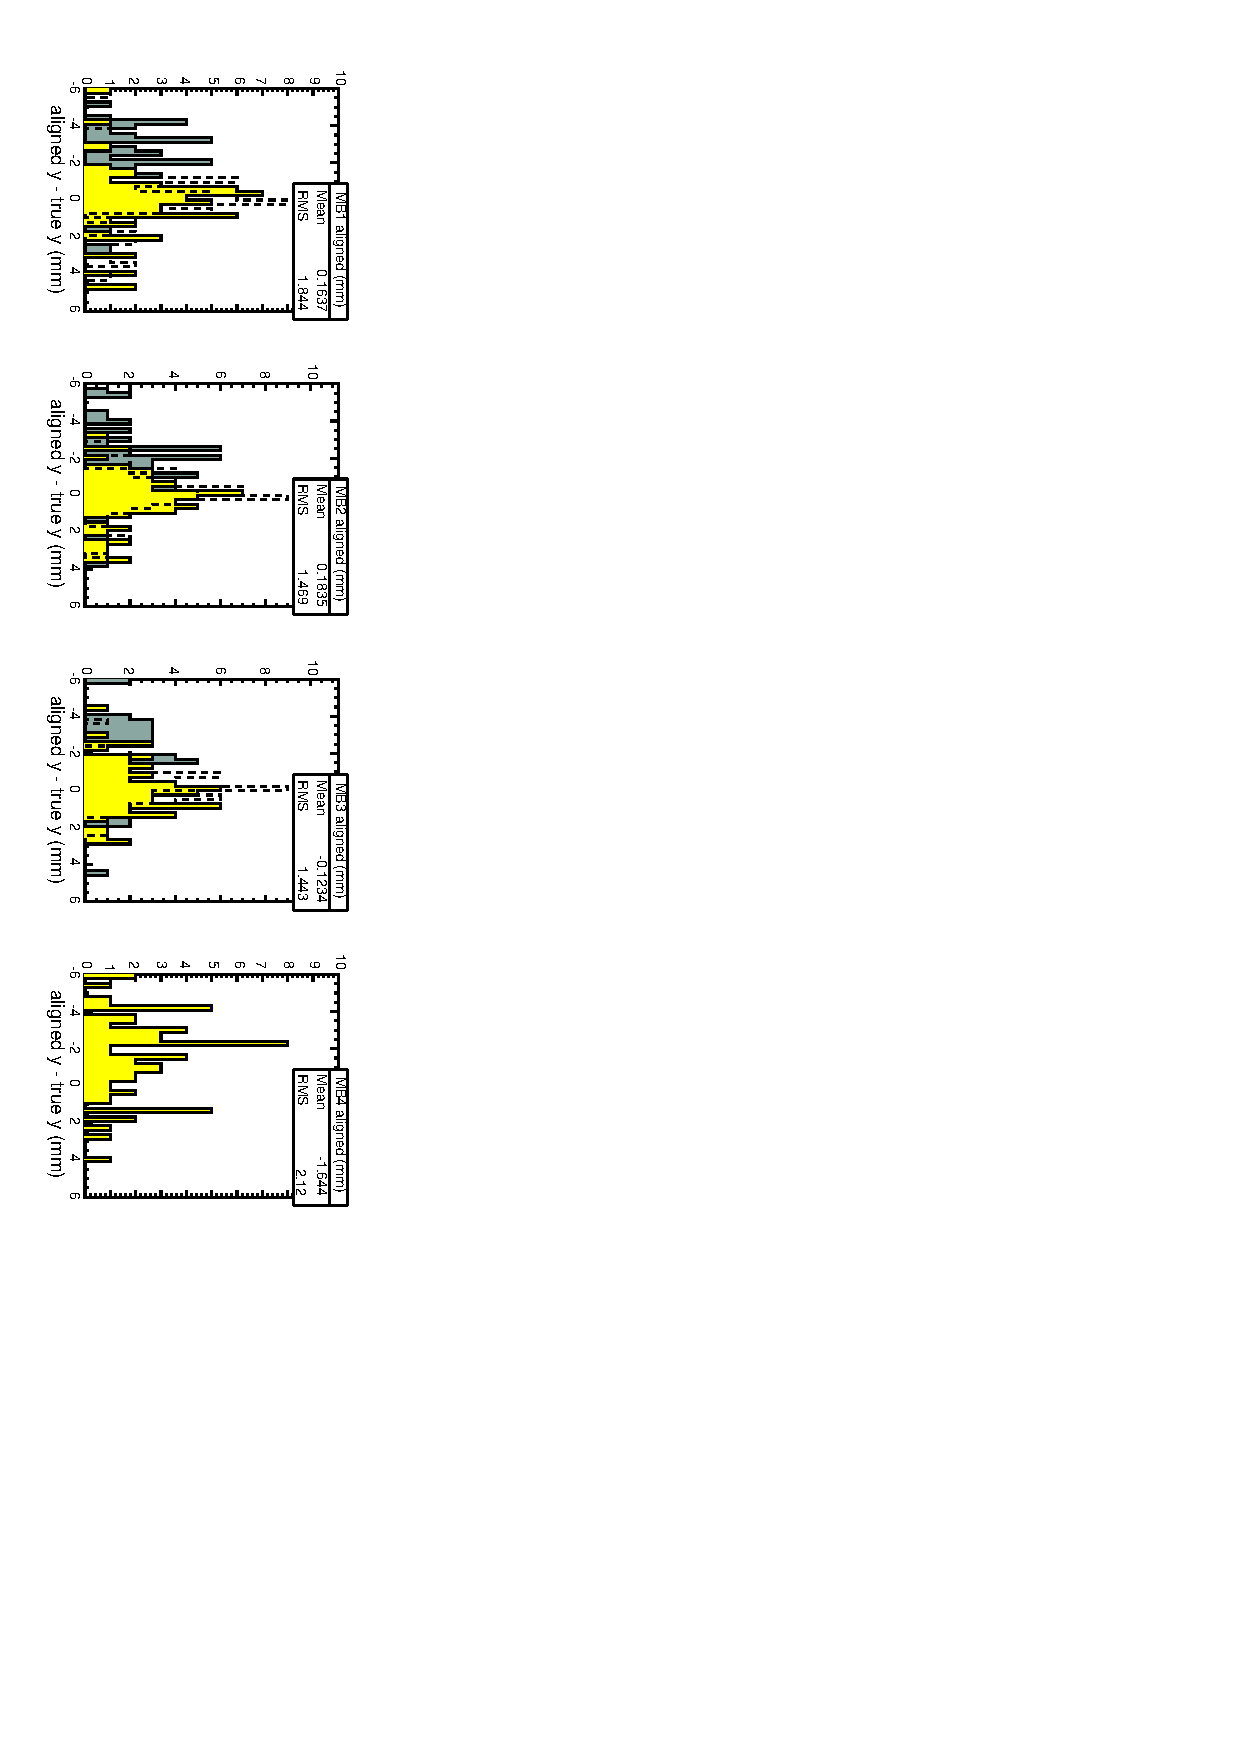
\includegraphics[height=\linewidth, angle=90]{S156_plots/muonhip_barrely.pdf}

\vfill
MillePede barrel station 1: 1870~$\mu$m

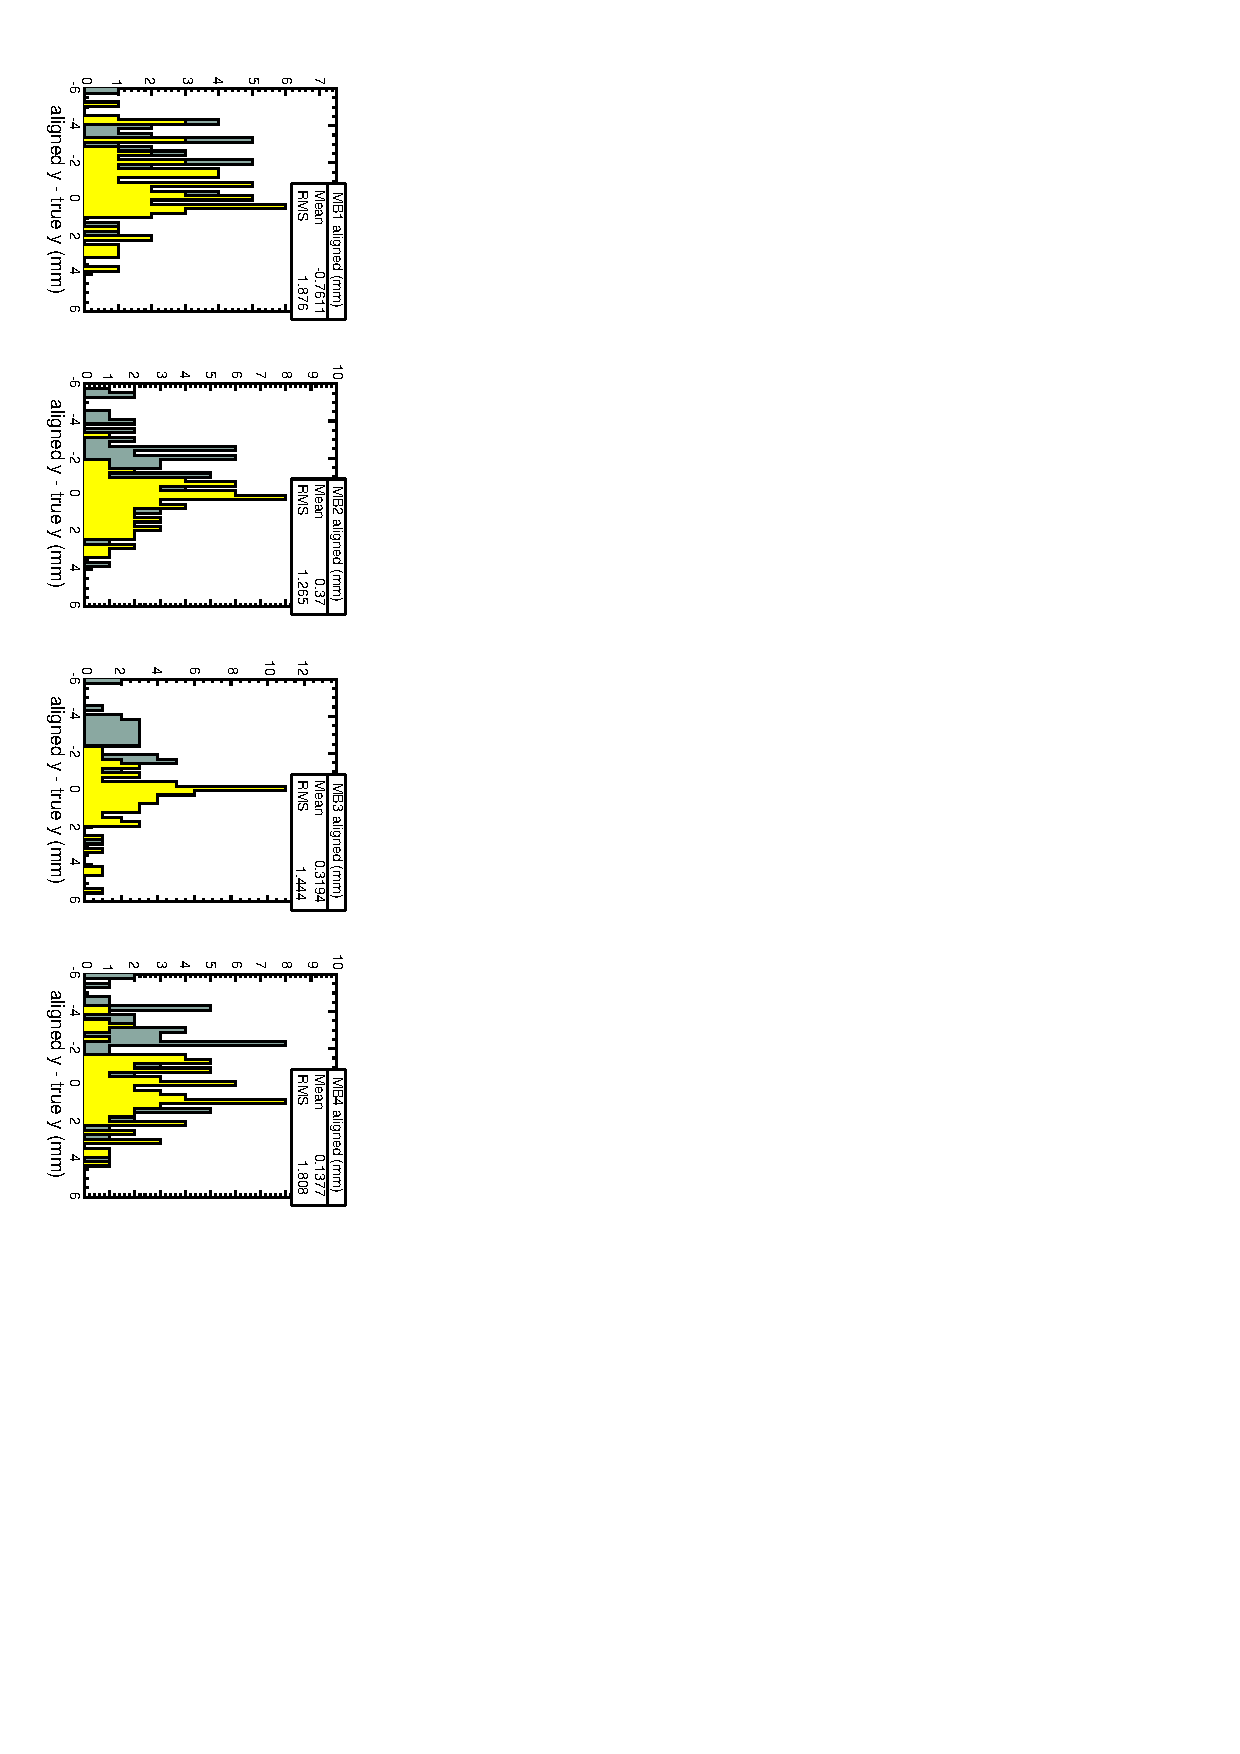
\includegraphics[height=\linewidth, angle=90]{S156_plots/millepede_barrely.pdf}

\vfill
Filled grey is initial misalignment, filled yellow is actual new constants, \\ dashed line if tracker were perfect
\end{frame}

\begin{frame}
\frametitle{Barrel comparison $\phi_z$}
\small

Muon HIP barrel actual station 1: 0.4~mrad

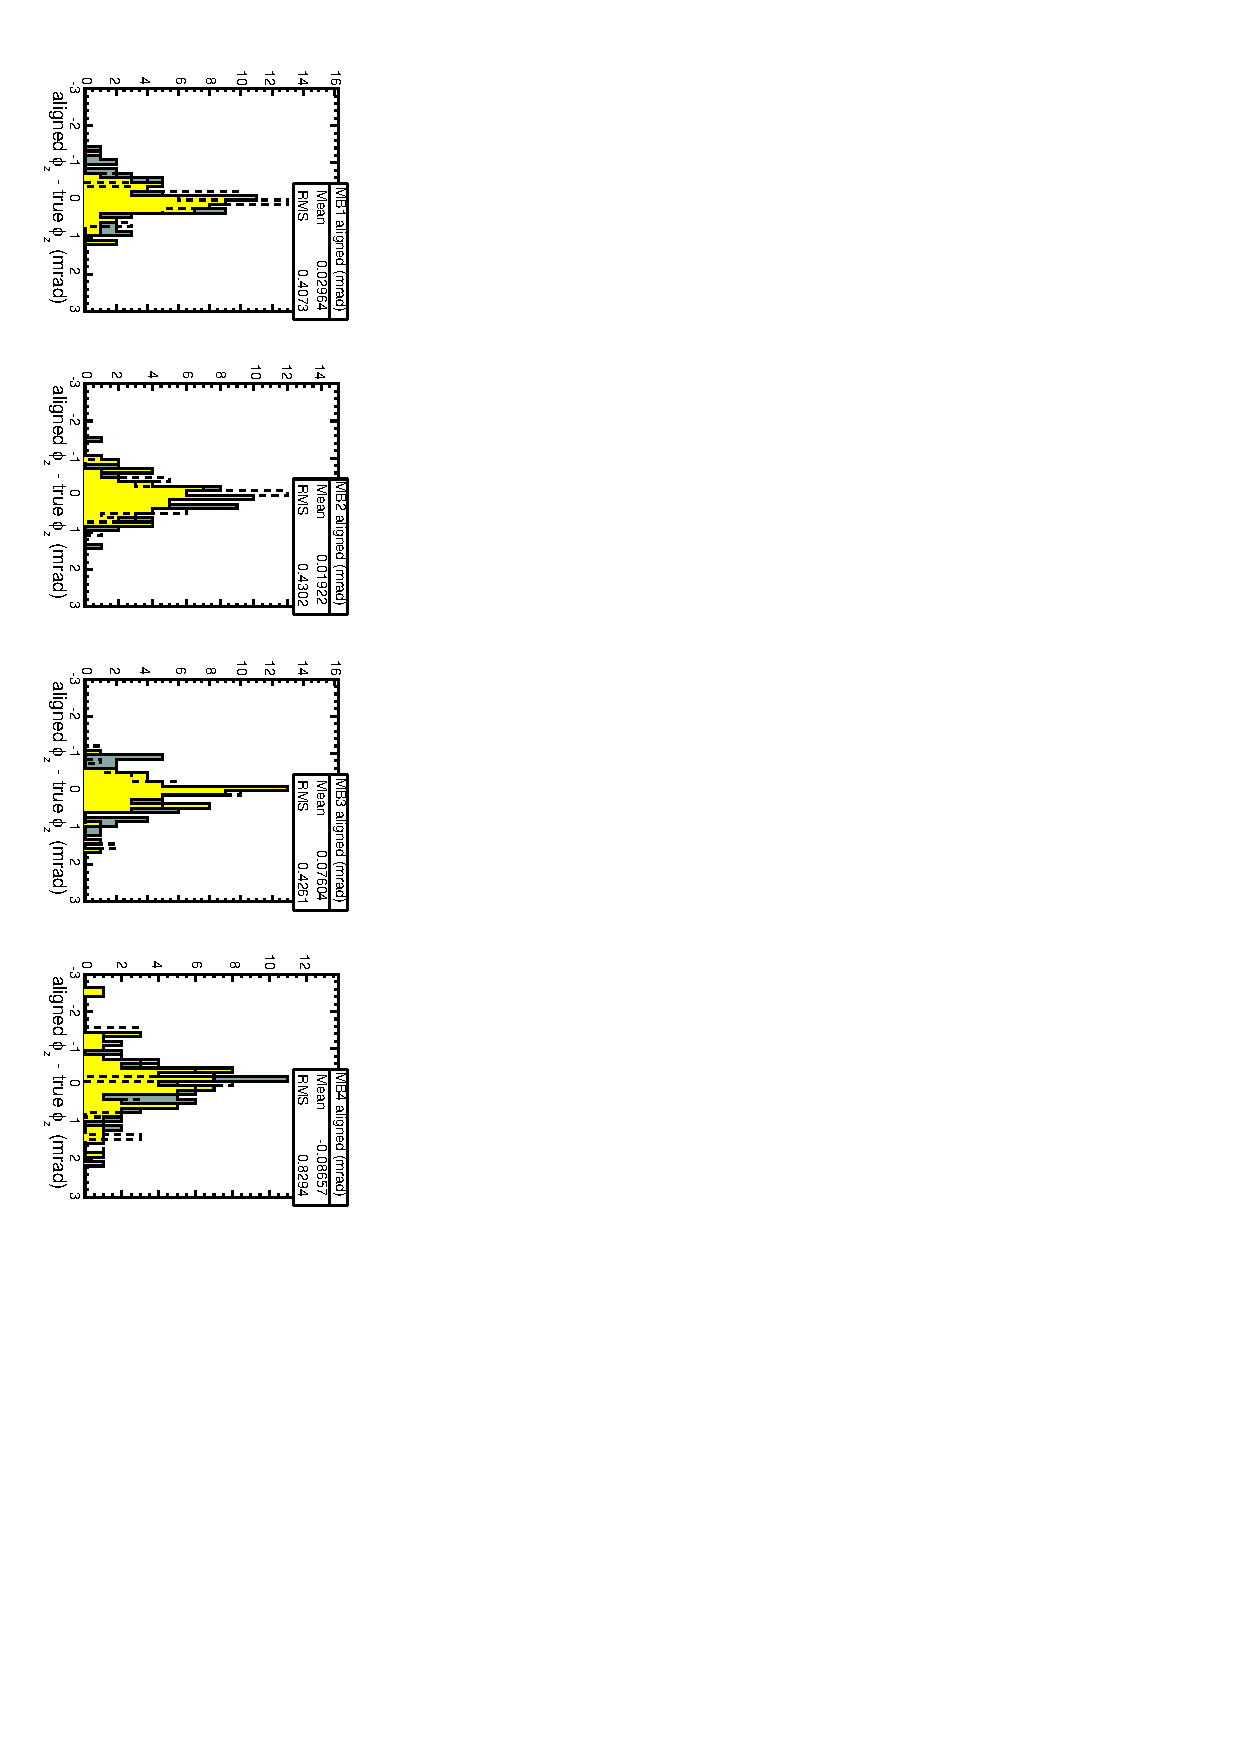
\includegraphics[height=\linewidth, angle=90]{S156_plots/muonhip_barrelphiz.pdf}

\vfill
MillePede barrel station 1: 0.6~mrad

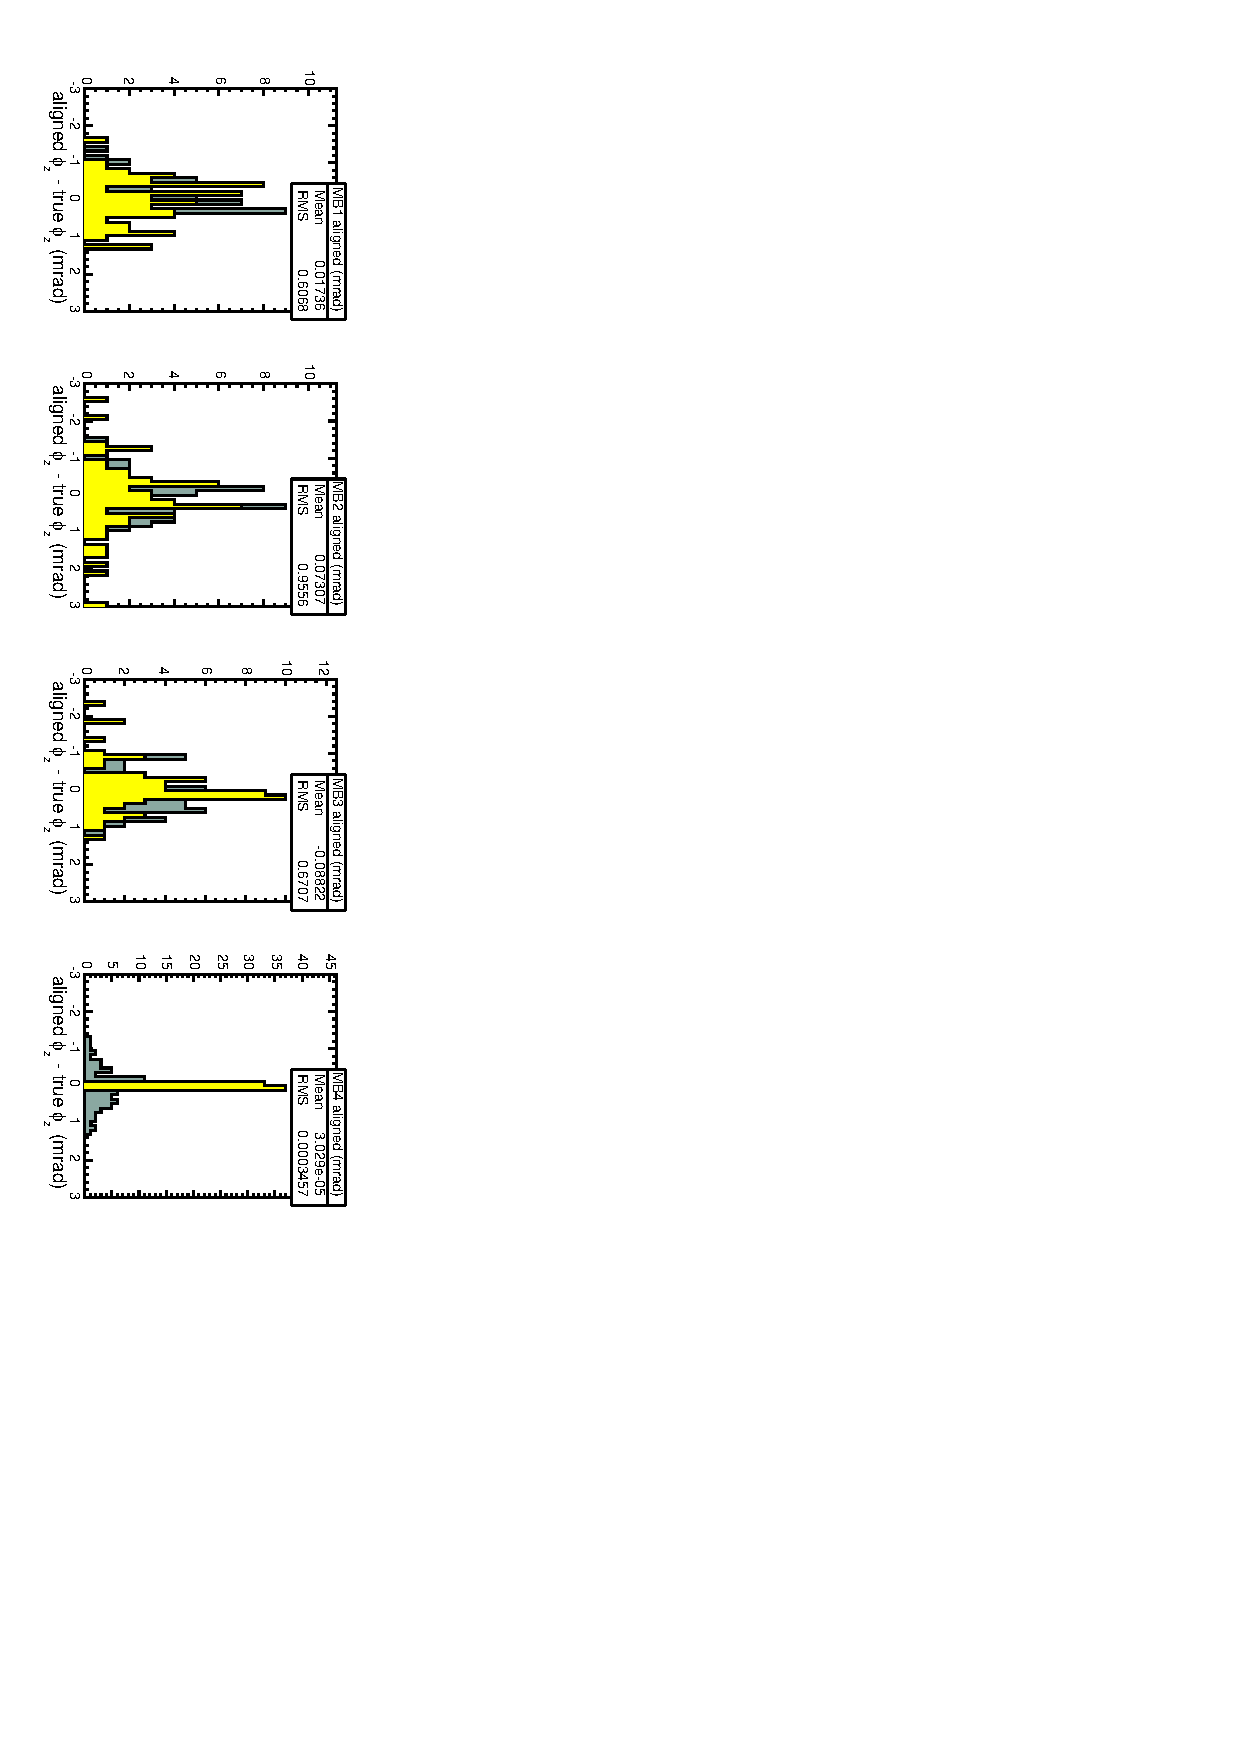
\includegraphics[height=\linewidth, angle=90]{S156_plots/millepede_barrelphiz.pdf}

\vfill
Filled grey is initial misalignment, filled yellow is actual new constants, \\ dashed line if tracker were perfect
\end{frame}

\begin{frame}
\frametitle{Endcap constants $x$ (global $r\phi$)}
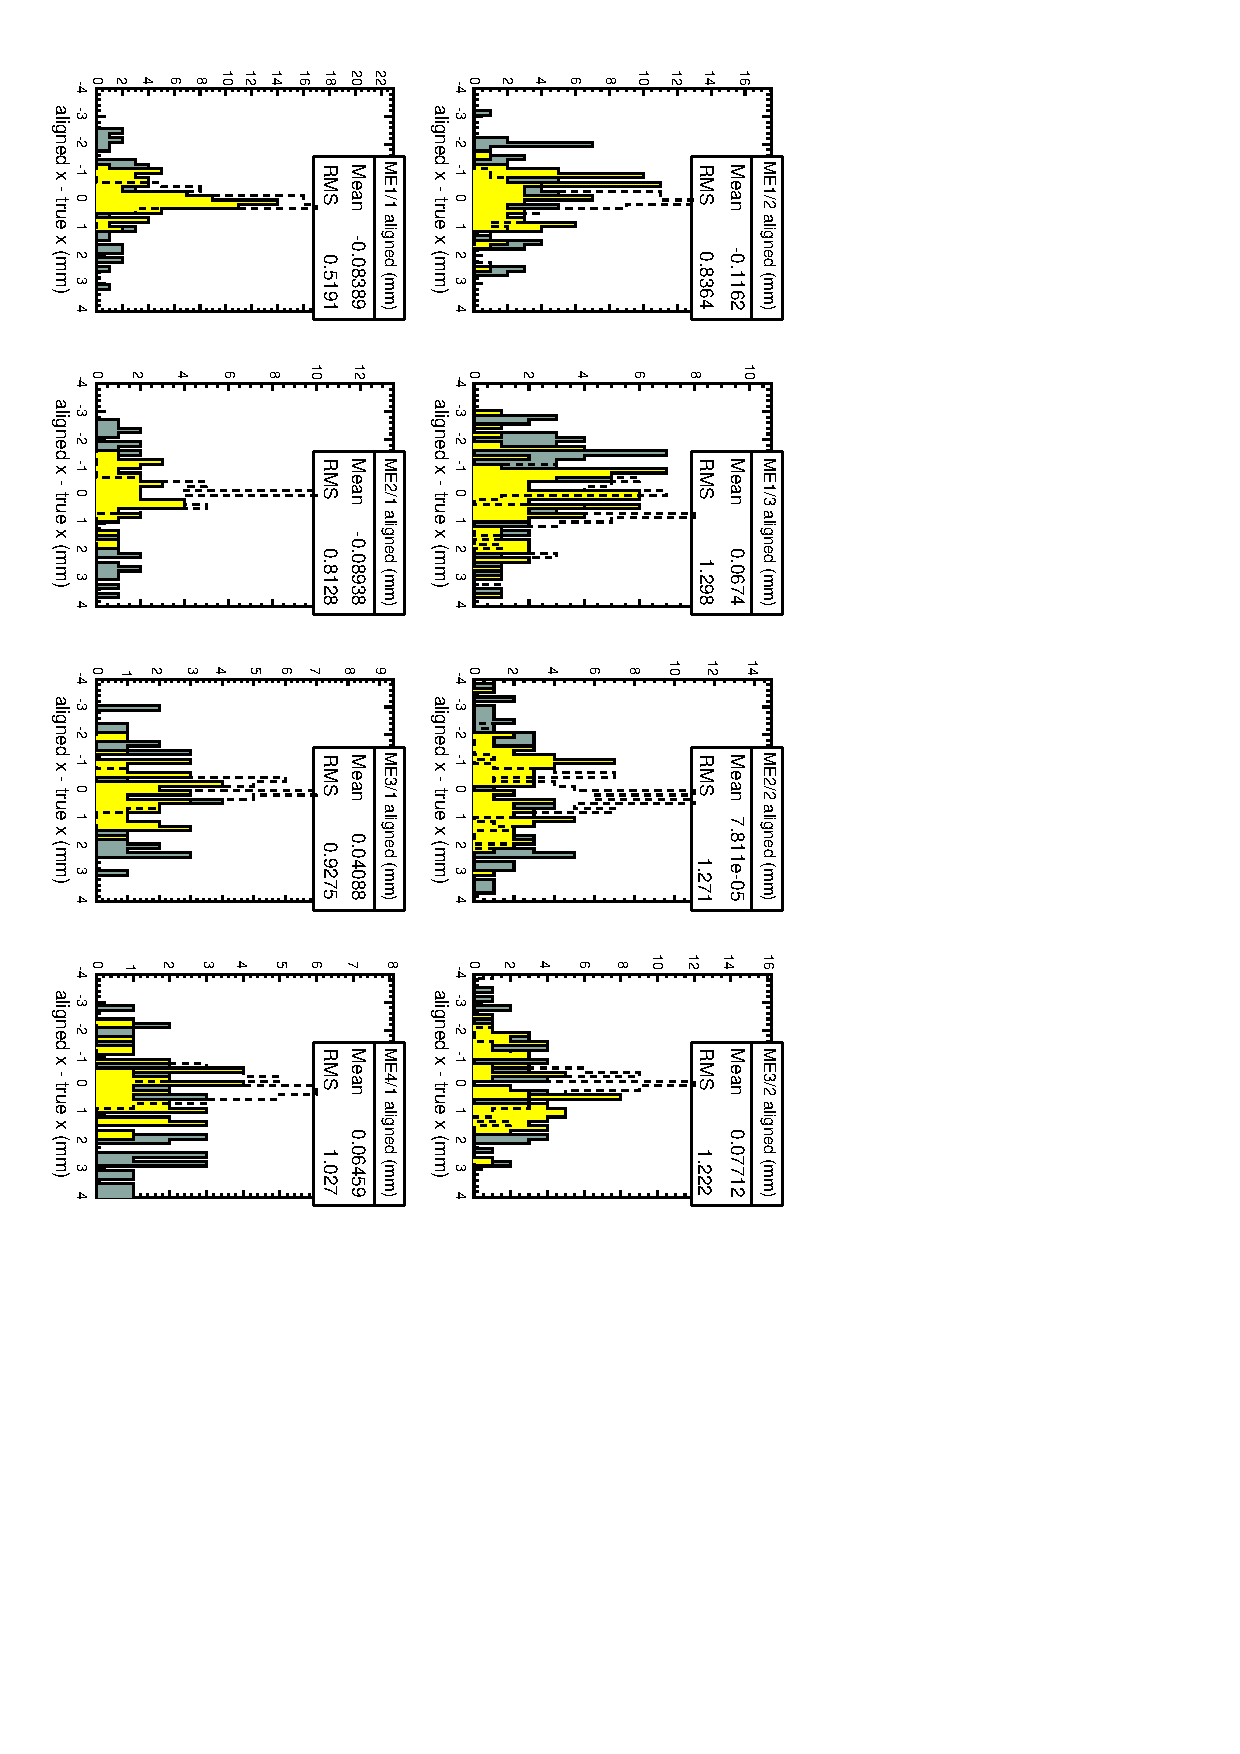
\includegraphics[height=\linewidth, angle=90]{S156_plots/muonhip_endcapx.pdf}
\end{frame}

\begin{frame}
\frametitle{Endcap constants $y$ (global $R$)}
\small

Best measurement where $p_T$ is small (inner ring); ME1/1 has an asymmetric $y$ residual distribution (under study)

\vfill
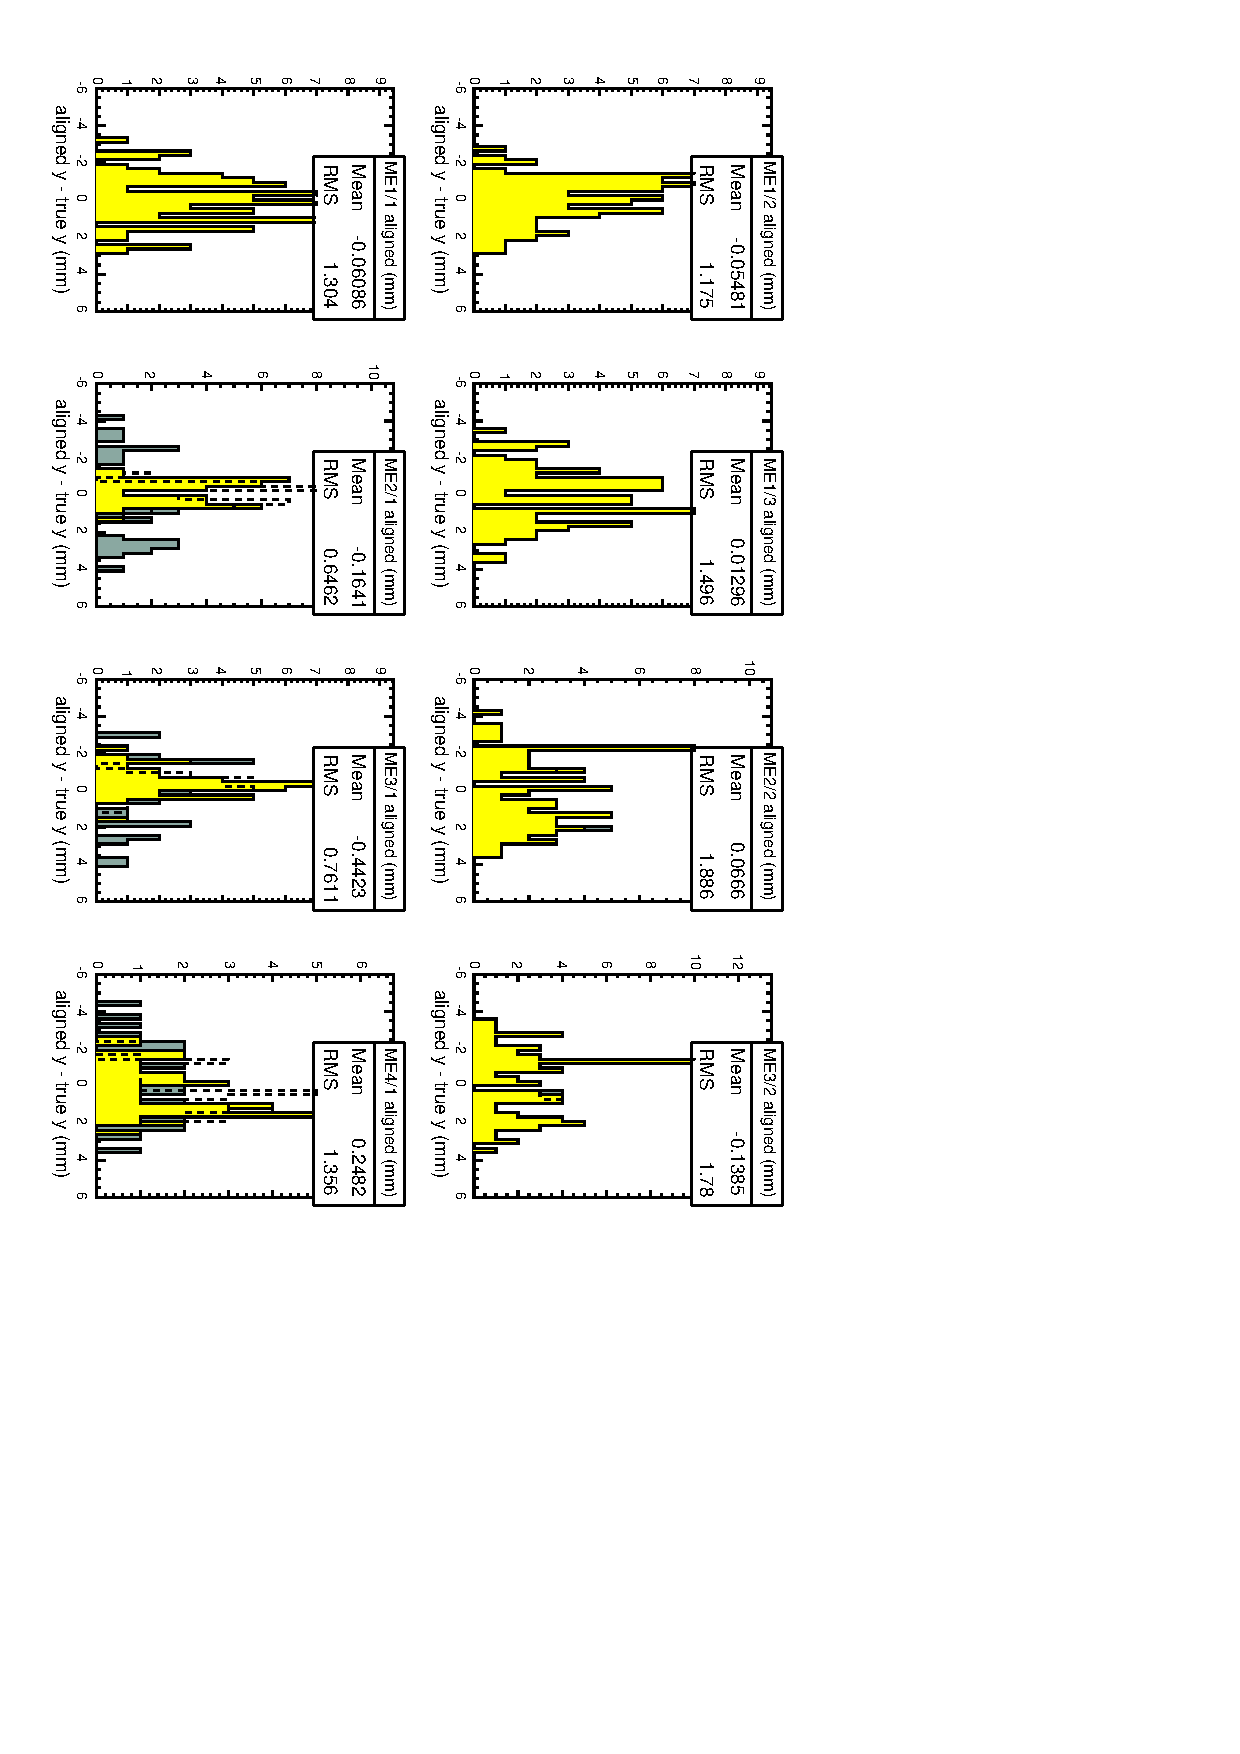
\includegraphics[height=\linewidth, angle=90]{S156_plots/muonhip_endcapy.pdf}
\end{frame}

\begin{frame}
\frametitle{Endcap constants $\phi_z$}
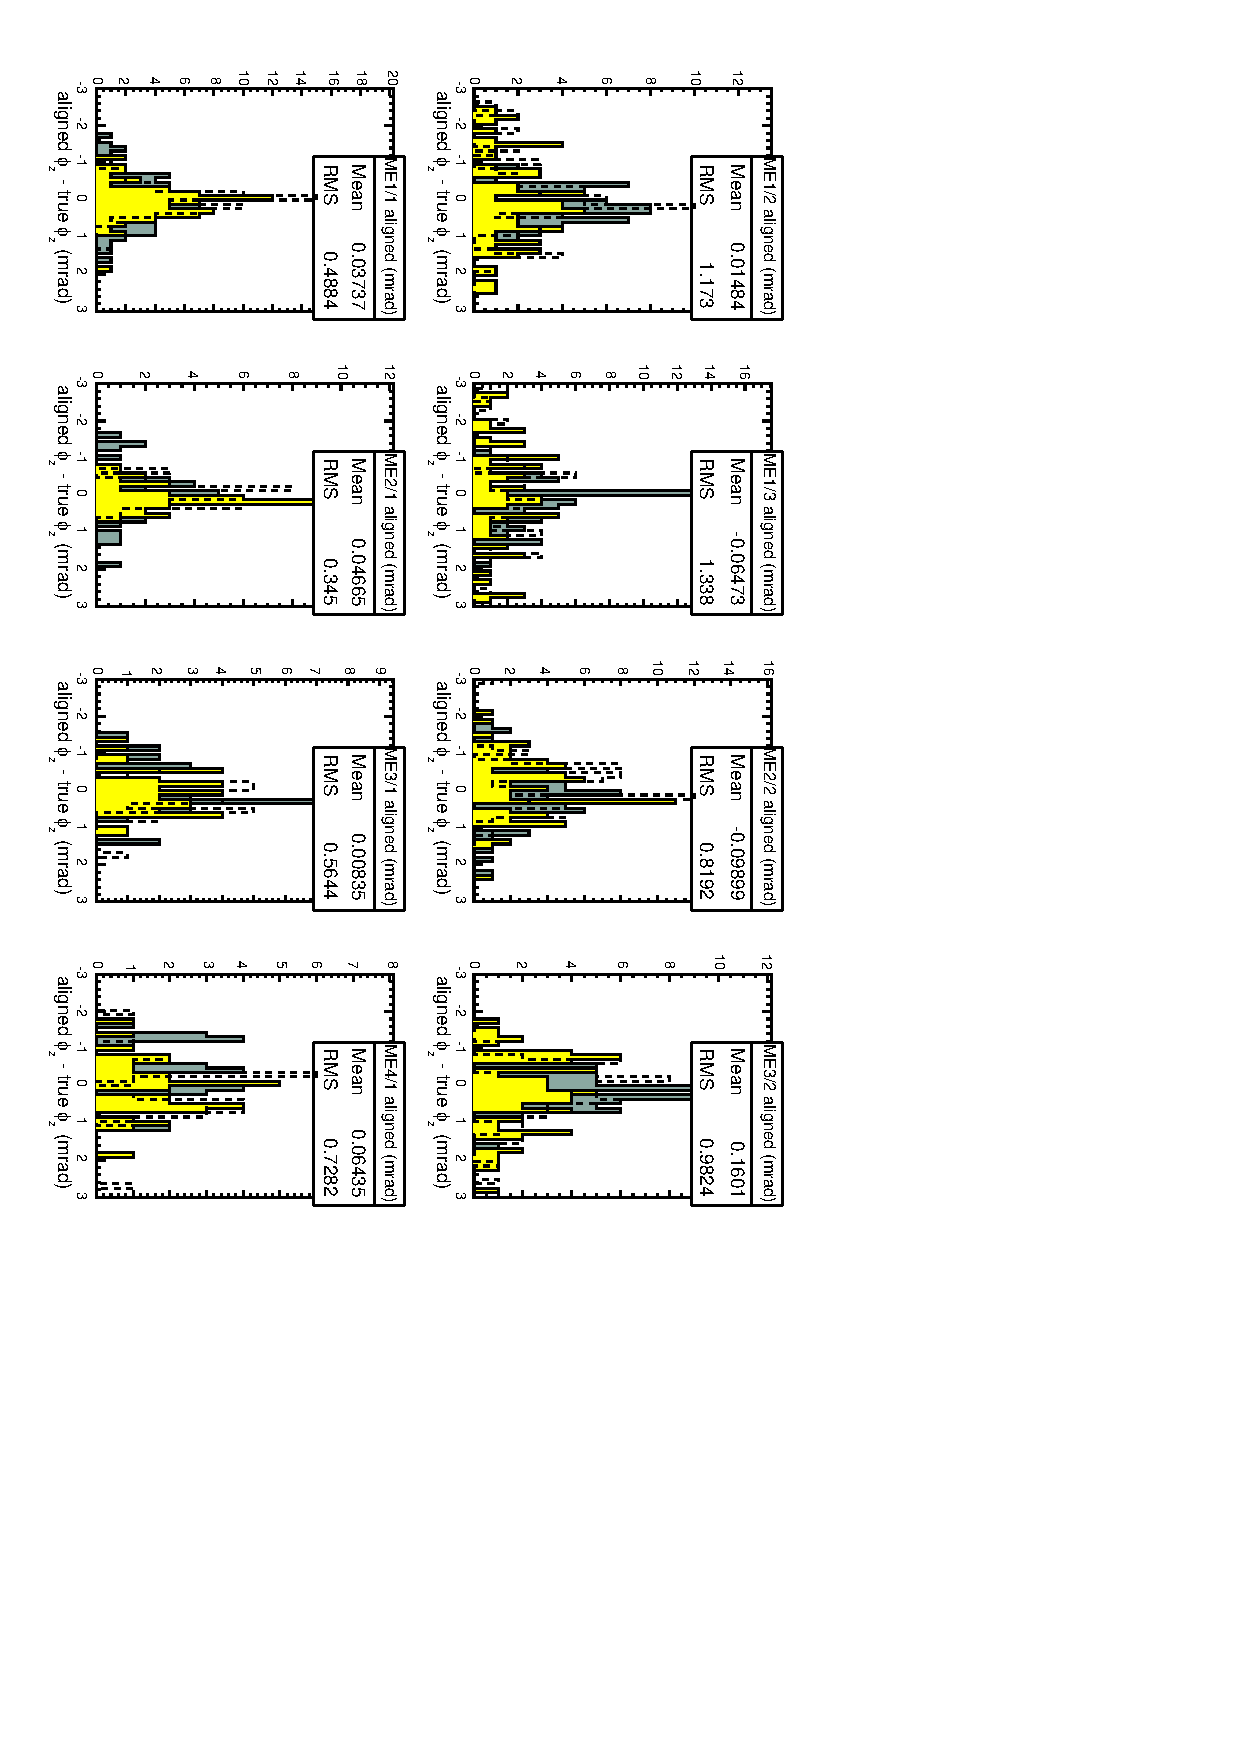
\includegraphics[height=\linewidth, angle=90]{S156_plots/muonhip_endcapphiz.pdf}
\end{frame}

\begin{frame}
\frametitle{Sanity check}
\small

Mean of residuals distributions, before (red) and after (blue) alignment

\vfill
Note: this is what I minimized

\vfill
\begin{columns}
\column{0.5\linewidth}
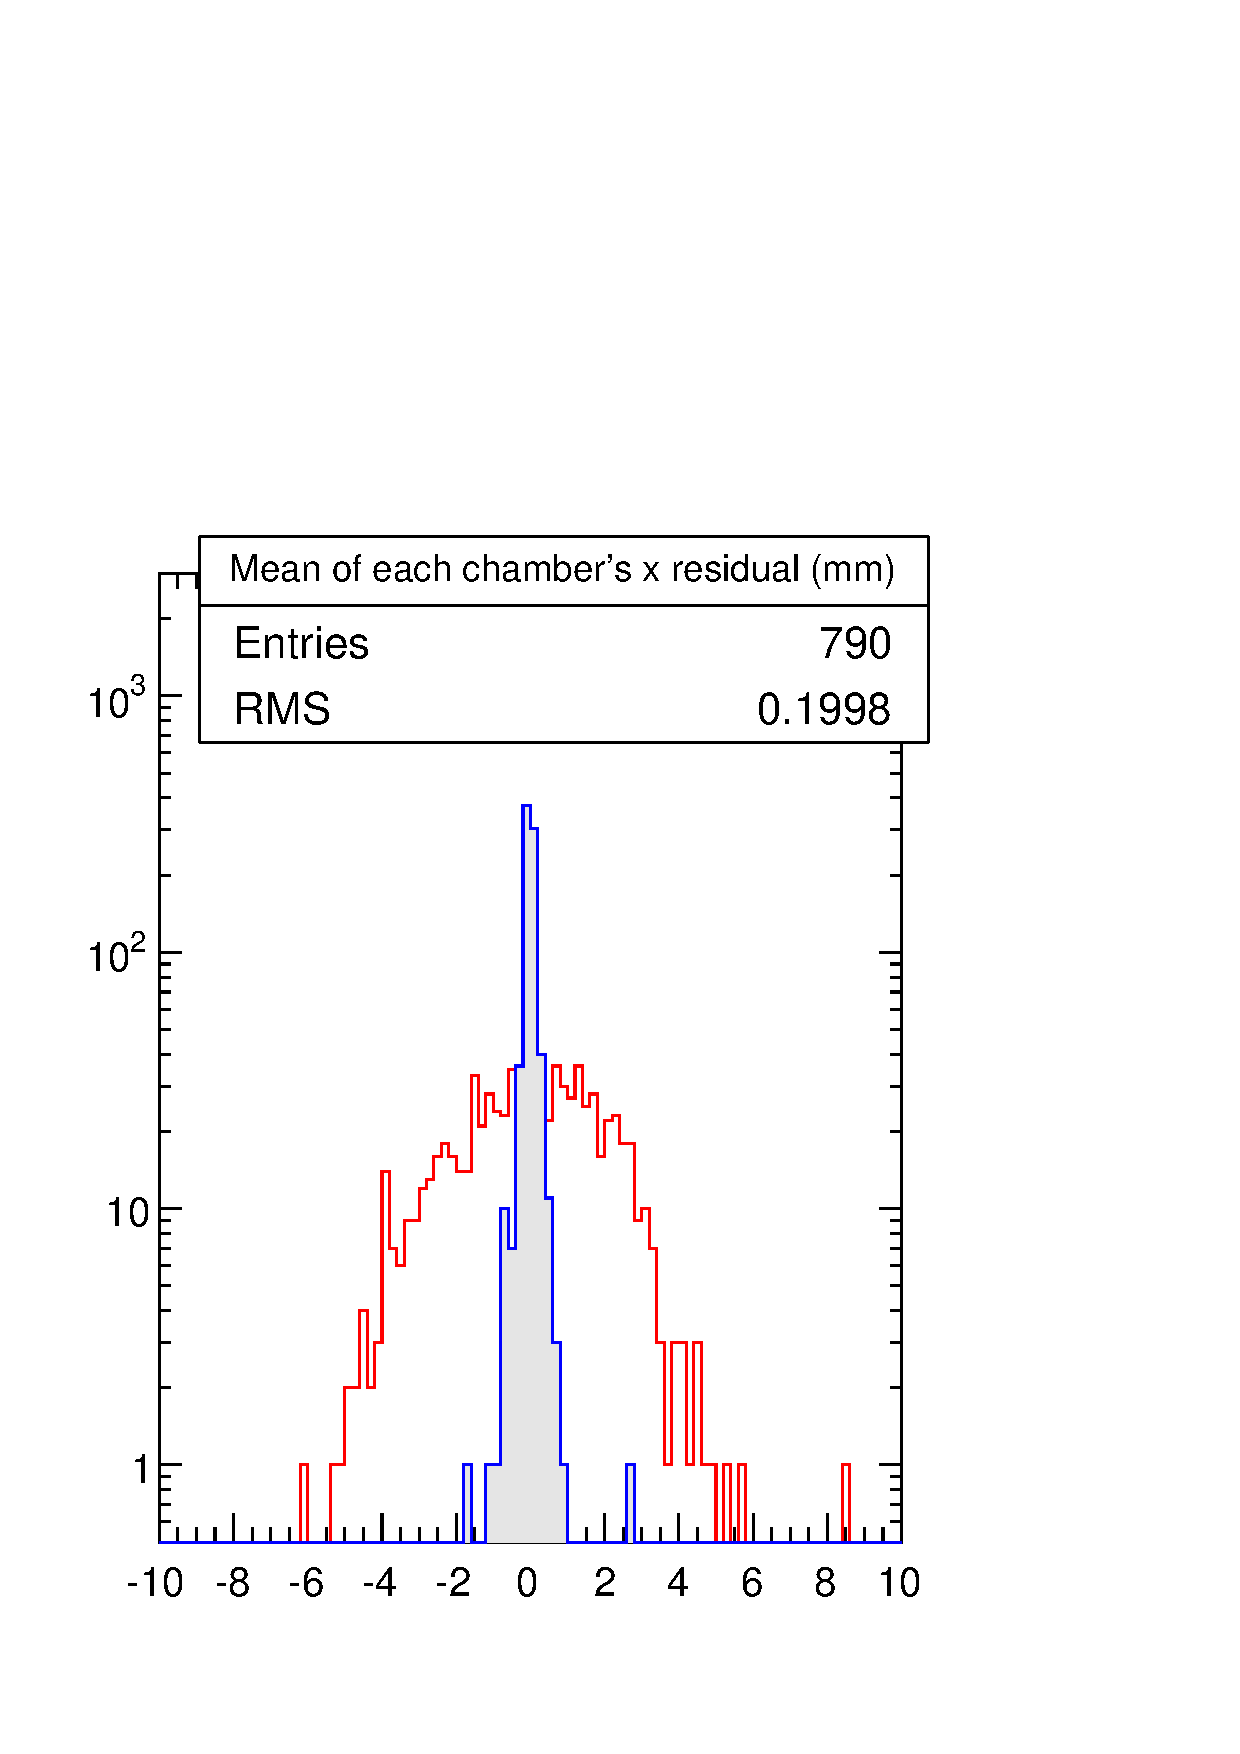
\includegraphics[width=\linewidth]{S156_plots/sanitycheck_x.pdf}
\column{0.5\linewidth}
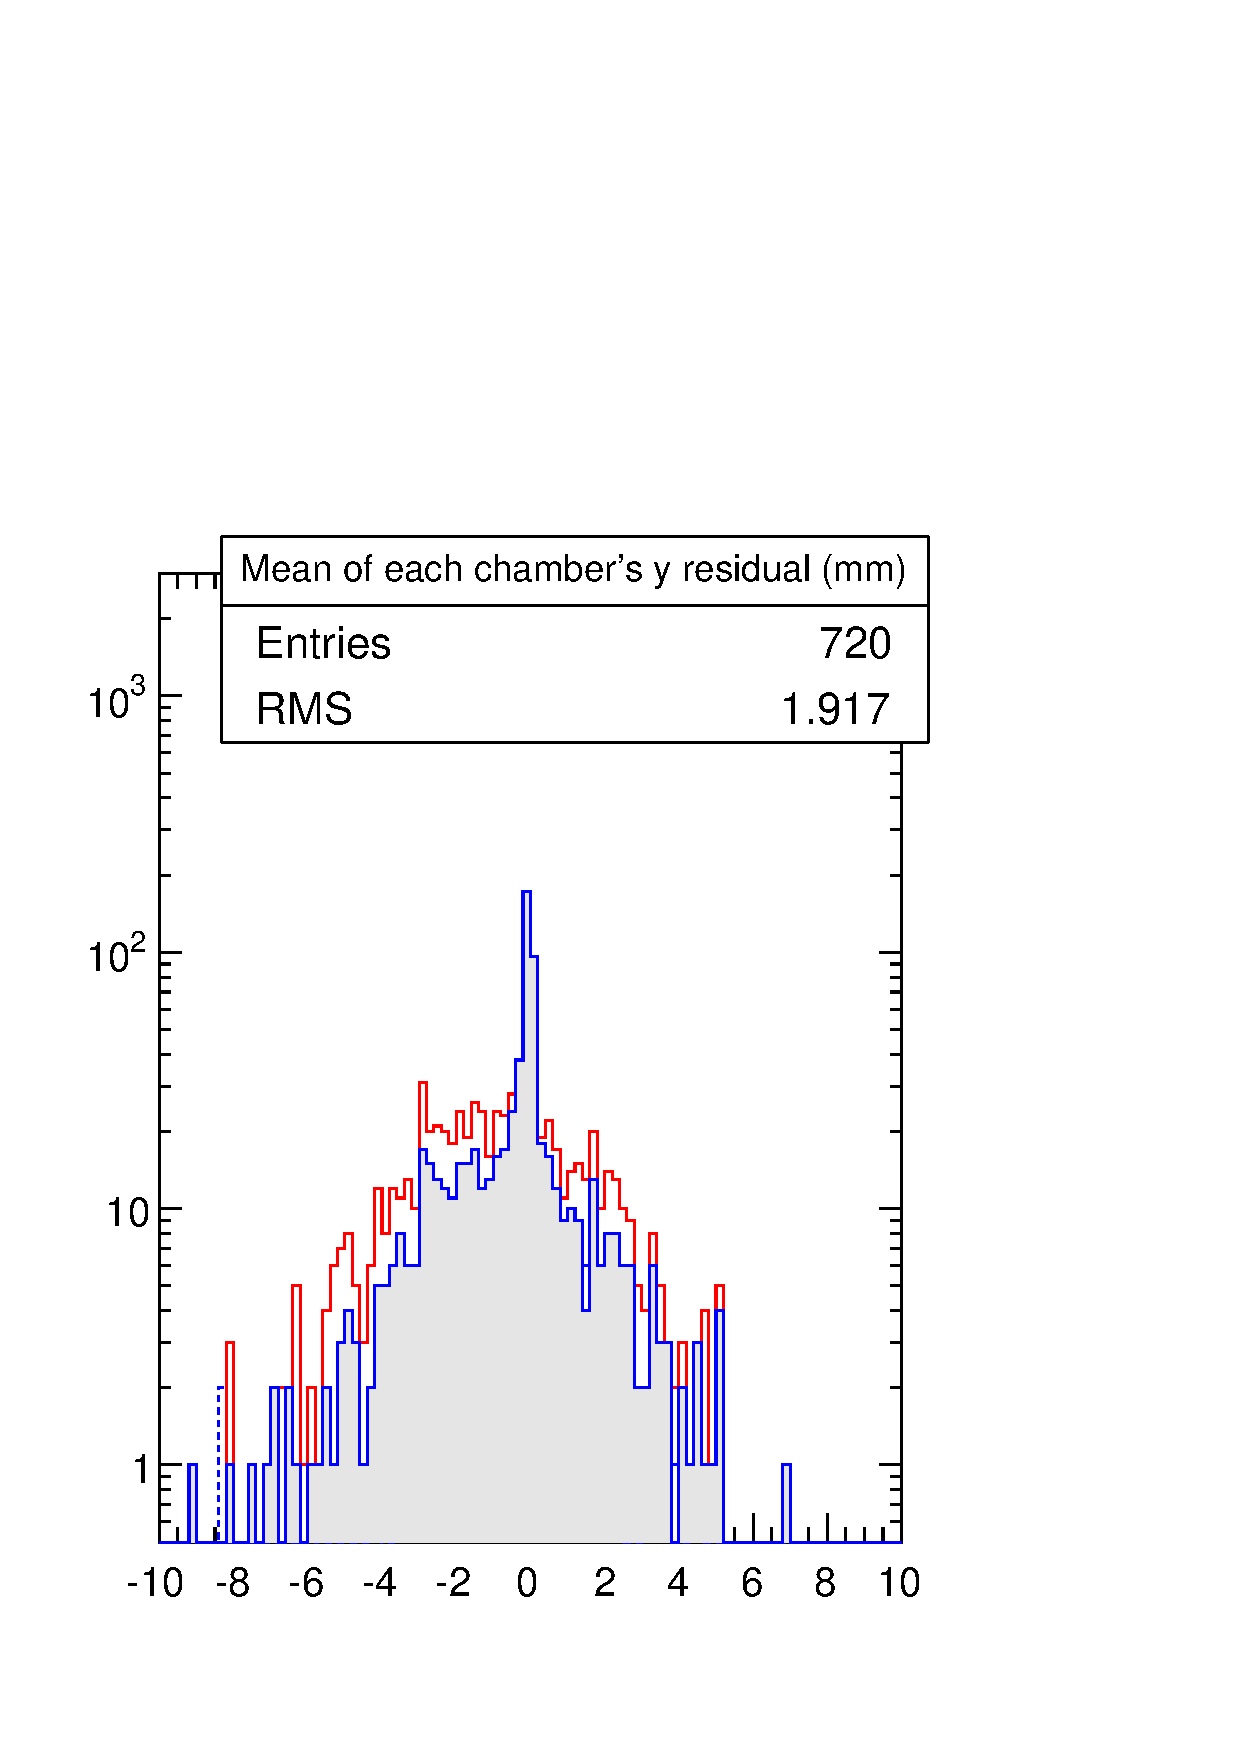
\includegraphics[width=\linewidth]{S156_plots/sanitycheck_y.pdf}
\end{columns}

\end{frame}

\begin{frame}
\frametitle{Figure of merit correlation}
\small

\vfill
Figure of merit ($\mbox{stdev}/\sqrt{N}$) correlated with sigma of alignment error

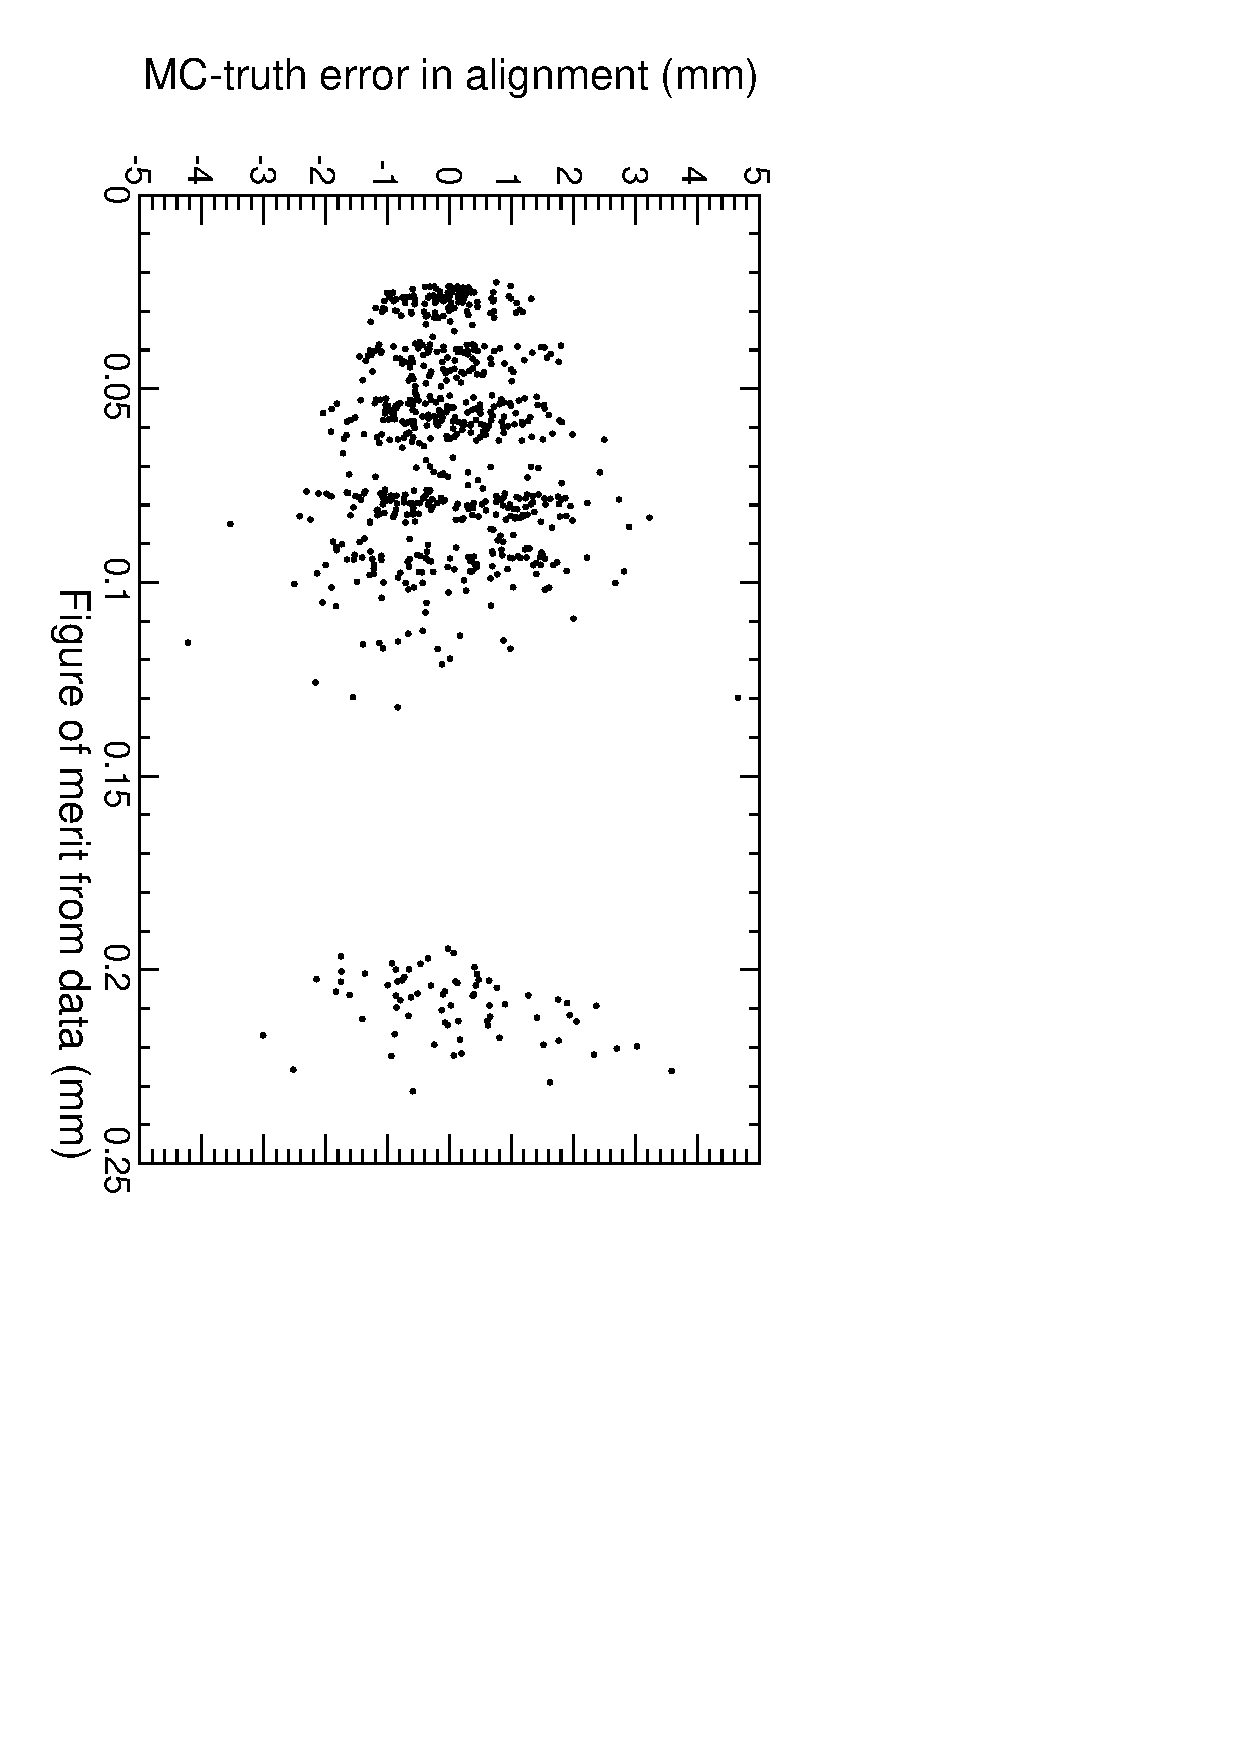
\includegraphics[height=\linewidth, angle=90]{correlation_trackerbest.pdf}
\end{frame}

%% \section*{First section}
%% \begin{frame}
%% \begin{center}
%% \Huge \textcolor{blue}{First section}
%% \end{center}
%% \end{frame}

\begin{frame}
\frametitle{Conclusions}

I recommend use of HIP constants for barrel and endcap

\vfill
To be taken offline:
\begin{itemize}
\item Perhaps tracker alignment can benefit from a weak constraint to muon hits
\item 1~cm APEs would tighten $p_T$ resolution without sensitivity to muon misalignment
\item improvement in tracker $p_T$ resolution would help muon alignment
\end{itemize}

\label{numpages}
\end{frame}

\end{document}
